\begin{table}[H]
    \centering
  \caption{Перелік деталей шасі}
    \begin{tabular}{|p{0.8cm}|p{3.2cm}|p{7.5cm}|p{2cm}|} 
        \hline
        \textbf{№} & \textbf{№ за каталогом} & \textbf{Найменування} & \textbf{Кількість} \\ \hline
        1 & 34560-189 & Бічна панель тип F, 3U, 295мм  & 2 од. \\ \hline
        2 & 34560-163 & Балка передня, тип L-KD, 84HP & 4 од. \\ \hline
        3 & 34560-463 & Балка задня, тип L-ST, 84HP & 2 од. \\ \hline
        4 & 24560-197 & Фланець тип F, 3U & 2 од. \\ \hline
        5 & 24561-198 & Задній профіль, 3U & 2 од. \\ \hline
        6 & 24560-073 & Панель EMC захисту , 84HP, 295мм & 2 од. \\ \hline
        7 & 34561-484 & Різьбова вставка M3*2*5 & 6 од. \\ \hline
        8 & 24560-233 & Планка ЕМС, 84НР & 4 шт. \\ \hline
        9 & 21100-646 & Гужон, М3х8 мм & 12 од. \\ \hline
       10 & 24560-130 & Гвинт з плоскою голівкою, Torx, M4 x 14 & 12 од. \\ \hline
       11 & 24560-135 & Гвинт з плоскою голівкою, Torx, M4 x 6 & 32 од. \\ \hline
       12 & 24560-140 & Гайка квадратна М4 & 13 од. \\ \hline
       13 & 34562-762 & Міжблоковий ЕМС екран, 220мм & 4 од. \\ \hline
       14 & 24560-353 & Напрямна, червона, 220мм & 18 од. \\ \hline
       15 & ISO7380-2 & Гвинт з напівкруглою голівкою та буртиком, оц.,10.9, М4х16 TORX,TX20 & 1 од. \\ \hline
       16 & DIN6798A & Шайба 4 стопорна A4 зовнішні зубці & 1 од. \\ \hline
       17 & DIN6727 AISI304 & Гайка з фланцем самоконтряща, M4 & 1 од. \\ \hline
       18 &  & Стійка шестигранна M3×7+8 MF, SW5, латунь. & 10 од. \\ \hline
       19 & ISO 7045 & Гвинт з напівкруглою головкою,M3×8 PH & 8 од. \\ \hline
       20 & ISO 7045 & Гвинт з напівкруглою головкою,M3×5 PH & 10 од. \\ \hline
       21 & ISO 7089 & Шайба плоска 3,оц. & 28 од. \\ \hline
       22 & DIN 127 B & Шайба пружинна розрізна 3 & 18 од. \\ \hline
       23 & KP DFZ 110.0226 & Кросплата & 1 од. \\ \hline
       24 & ЕПМ7.001.016 & Екран КР-210 SCHROFF & 1 од. \\ \hline
   
    \end{tabular}
    
\end{table}

\begin{figure}[H]
    \centering
    % Переконайтеся, що файл зображення завантажений в Overleaf
    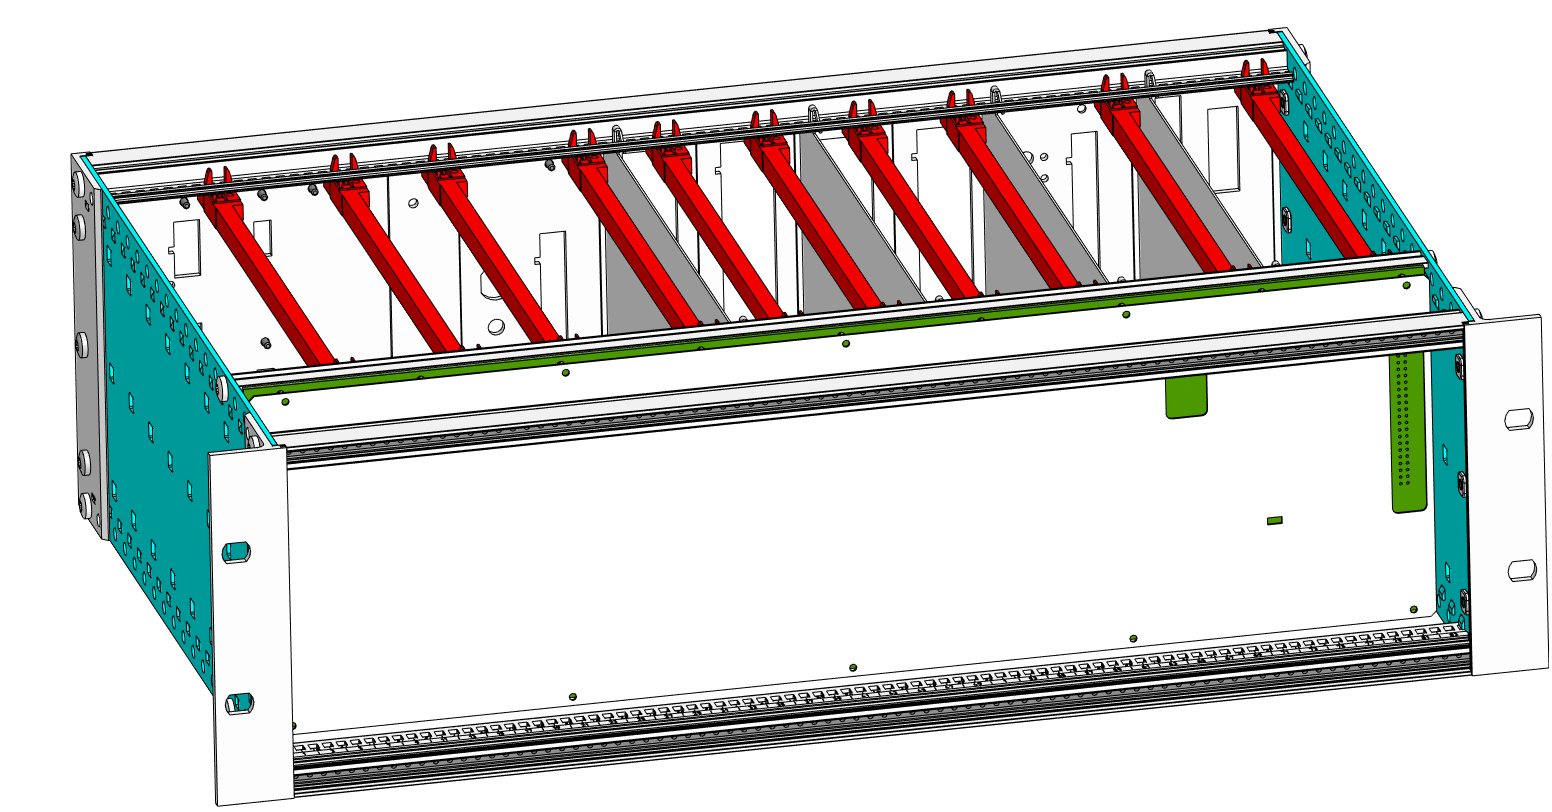
\includegraphics[width=1.0\textwidth]{images/A68.png} 
   % \caption{ОРІОН УПЗА}
\end{figure}
\begin{figure}[H]
    \centering
    % Переконайтеся, що файл зображення завантажений в Overleaf
    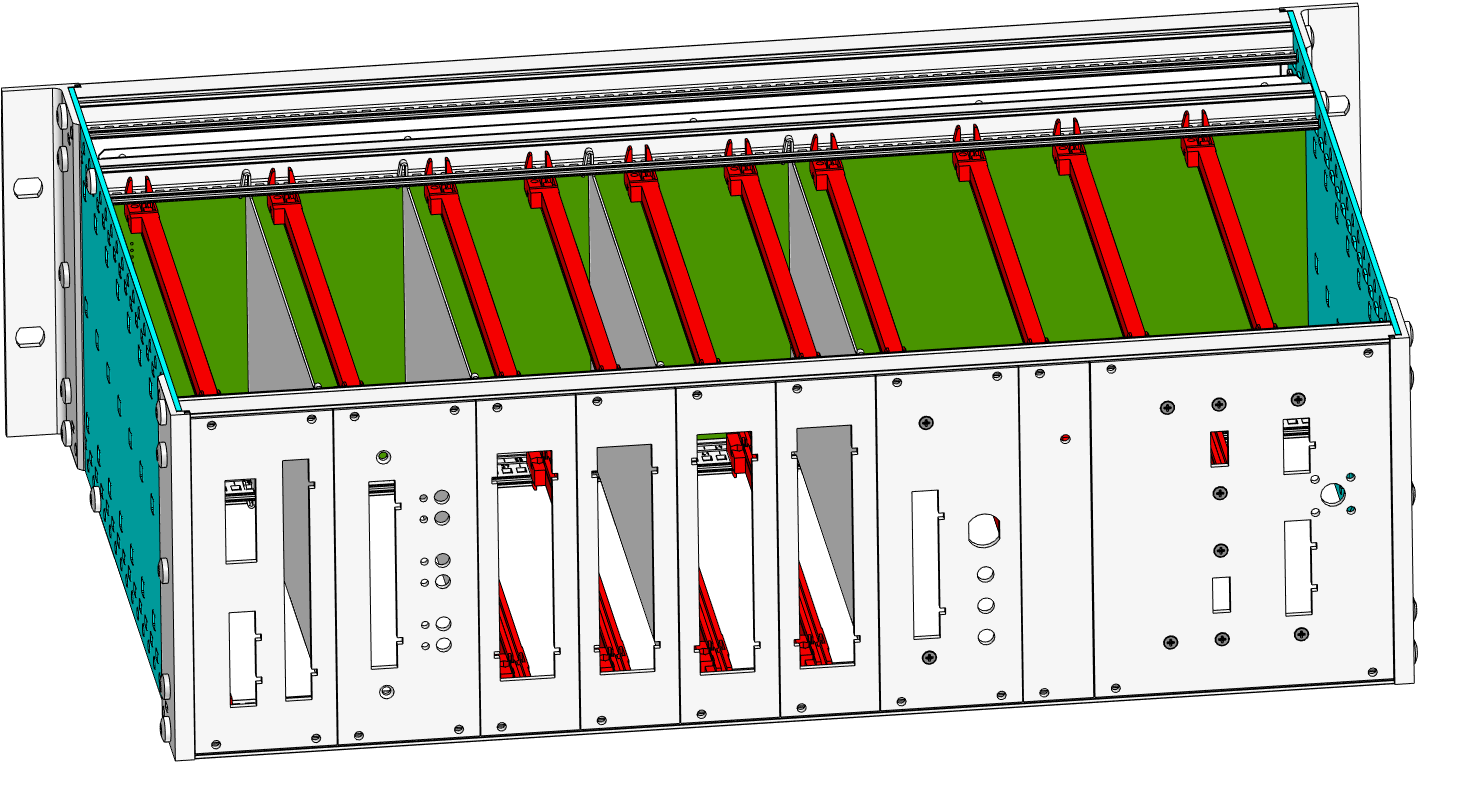
\includegraphics[width=1.0\textwidth]{images/A69.png} 
    \caption{ОРІОН УПЗА}
\end{figure}

\begin{mybox}{Важливо}
Розташування екранів: 1/9, 2/20, 3/33, 4/47
\end{mybox}

\begin{mybox}{Важливо}
Розташування напрямних: 1/2, 2/12, 3/23, 4/30, 5/37, 6/44, 7/49, 8/60, 9/67, 10/76
\end{mybox}
